\newcommand\drawrectangle[6]{
  \draw[#5, thick, fill=#5!30, opacity=.8] (#1, #2) rectangle ++(#3, #4);%
  \fill[#5] (#1, #2) circle (.2cm);
  \node[#5] at ({#1 + #3/2}, {#2 + #4/2}) {#6};
}

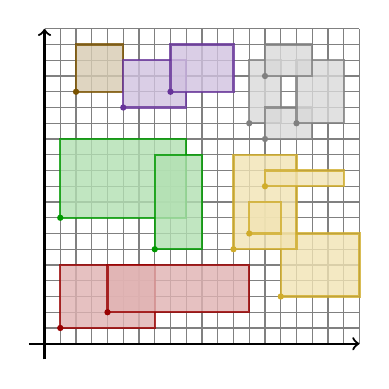
\begin{tikzpicture}[scale=.2]

  \def\gridsize{20}
  \draw[gray] (0, 0) grid (\gridsize, \gridsize);
  \draw[thick,->] (-1, 0) -- (\gridsize, 0);
  \draw[thick,->] (0, -1) -- (0, \gridsize);

  \drawrectangle{ 1}{ 8}{8}{5}{green!60!black}{}
  \drawrectangle{ 7}{ 6}{3}{6}{green!60!black}{}
  \drawrectangle{ 1}{ 1}{6}{4}{red!60!black}{}
  \drawrectangle{ 4}{ 2}{9}{3}{red!60!black}{}
  \drawrectangle{15}{ 3}{5}{4}{yellow!80!red!80!black}{}
  \drawrectangle{12}{ 6}{4}{6}{yellow!80!red!80!black}{}
  \drawrectangle{14}{10}{5}{1}{yellow!80!red!80!black}{}
  \drawrectangle{13}{ 7}{2}{2}{yellow!80!red!80!black}{}
  \drawrectangle{ 2}{16}{3}{3}{red!60!green!80!black}{}
  \drawrectangle{ 5}{15}{4}{3}{blue!60!orange}{}
  \drawrectangle{ 8}{16}{4}{3}{blue!60!orange}{}
  \drawrectangle{13}{14}{2}{4}{gray}{}
  \drawrectangle{14}{13}{3}{2}{gray}{}
  \drawrectangle{16}{14}{3}{4}{gray}{}
  \drawrectangle{14}{17}{3}{2}{gray}{}

  %\foreach\i in {0,...,\gridsize} {
  %    \node[gray] at (\i, -.5) {\i};
  %    \node[gray] at (-.5, \i) {\i};
  %}

\end{tikzpicture}

